%%%%%%%%%%%%%%%%%%%%%%%%%%%%%%%%%%%%%%%%%
% Oliver Lemon made minor edits (jan 2015)  to : 
% Masters/Doctoral Thesis 
% LaTeX Template
% Version 1.43 (17/5/14)
%
% This template has been downloaded from:
% http://www.LaTeXTemplates.com
%
% Original authors:
% Steven Gunn 
% http://users.ecs.soton.ac.uk/srg/softwaretools/document/templates/
% and
% Sunil Patel
% http://www.sunilpatel.co.uk/thesis-template/
%
% License:
% CC BY-NC-SA 3.0 (http://creativecommons.org/licenses/by-nc-sa/3.0/)
%
% Note:
% Make sure to edit document variables in the Thesis.cls file
%
%%%%%%%%%%%%%%%%%%%%%%%%%%%%%%%%%%%%%%%%%

%----------------------------------------------------------------------------------------
%	PACKAGES AND OTHER DOCUMENT CONFIGURATIONS
%----------------------------------------------------------------------------------------

\documentclass[11pt, oneside]{Thesis} % The default font size and one-sided printing (no margin offsets)

\graphicspath{{Pictures/}} % Specifies the directory where pictures are stored

\usepackage[square, comma, sort&compress]{natbib} % Use the natbib reference package - read up on this to edit the reference style; if you want text (e.g. Smith et al., 2012) for the in-text references (instead of numbers), remove 'numbers' 
\setcitestyle{numbers}

\hypersetup{urlcolor=blue, colorlinks=true} % Colors hyperlinks in blue - change to black if annoying

\usepackage{todonotes}
\usepackage{float}


\title{HWU CS Masters thesis template} % BUT you should use use " \title{\ttitle} " here instead to define the thesis title ! 
% \ttitle is defined in the file Thesis.cls 

\begin{document}

\frontmatter % Use roman page numbering style (i, ii, iii, iv...) for the pre-content pages

\setstretch{1.3} % Line spacing of 1.3

% Define the page headers using the FancyHdr package and set up for one-sided printing
\fancyhead{} % Clears all page headers and footers
\rhead{\thepage} % Sets the right side header to show the page number
\lhead{} % Clears the left side page header

\pagestyle{fancy} % Finally, use the "fancy" page style to implement the FancyHdr headers

\newcommand{\HRule}{\rule{\linewidth}{0.5mm}} % New command to make the lines in the title page

% PDF meta-data
\hypersetup{pdftitle={\ttitle}}
\hypersetup{pdfsubject=\subjectname}
\hypersetup{pdfauthor=\authornames}
\hypersetup{pdfkeywords=\keywordnames}

%----------------------------------------------------------------------------------------
%	TITLE PAGE
%----------------------------------------------------------------------------------------

\begin{titlepage}
\begin{center}

\textsc{\LARGE \univname}\\[1.5cm] % University name
\textsc{\Large Masters Thesis}\\[0.5cm] % Thesis type

\HRule \\[0.4cm] % Horizontal line
{\huge \bfseries \ttitle}\\[0.4cm] % Thesis title
\HRule \\[1.5cm] % Horizontal line
 
\begin{minipage}{0.4\textwidth}
\begin{flushleft} \large
\emph{Author:}\\
\href{http://www.johnsmith.com}{\authornames} % Author name - remove the \href bracket to remove the link
\end{flushleft}
\end{minipage}
\begin{minipage}{0.4\textwidth}
\begin{flushright} \large
\emph{Supervisor:} \\
\href{http://www.jamessmith.com}{\supname} % Supervisor name - remove the \href bracket to remove the link  
\end{flushright}
\end{minipage}\\[3cm]
 
\large \textit{A thesis submitted in fulfilment of the requirements\\ for the degree of \degreename}\\[0.3cm] % University requirement text
\textit{in the}\\[0.4cm]
%\groupname\\

\deptname\\[2cm] % Research group name and department name
 
{\large \today}\\[1cm] % Date

\includegraphics[width=6cm]{./Figures/HWUlogo.jpg} % University/department logo - uncomment to place it
 
\vfill
\end{center}

\end{titlepage}

%----------------------------------------------------------------------------------------
%	DECLARATION PAGE
%	Your institution may give you a different text to place here
%----------------------------------------------------------------------------------------

\Declaration{

\addtocontents{toc}{\vspace{1em}} % Add a gap in the Contents, for aesthetics

I, \authornames, declare that this thesis titled, '\ttitle' and the work presented in it is my own. I confirm that this work submitted for assessment is my own and is
  expressed in my own words. Any uses made within it of the works of
  other authors in any form (e.g., ideas, equations, figures, text,
  tables, programs) are properly acknowledged at any point of their
  use. A list of the references employed is included.

%\begin{itemize} 
%\item[\tiny{$\blacksquare$}] This work was done wholly or mainly while in candidature for a research degree at this University.
%\item[\tiny{$\blacksquare$}] Where any part of this thesis has previously been submitted for a degree or any other qualification at %this University or any other institution, this has been clearly stated.
%\item[\tiny{$\blacksquare$}] Where I have consulted the published work of others, this is always clearly attributed.
%\item[\tiny{$\blacksquare$}] Where I have quoted from the work of others, the source is always given. With the exception of such %quotations, this thesis is entirely my own work.
%\item[\tiny{$\blacksquare$}] I have acknowledged all main sources of help.
%\item[\tiny{$\blacksquare$}] Where the thesis is based on work done by myself jointly with others, I have made clear exactly what %was done by others and what I have contributed myself.\\
%\end{itemize}
 \vspace{2cm} 
Signed:\\
\rule[1em]{25em}{0.5pt} % This prints a line for the signature
 
Date:\\
\rule[1em]{25em}{0.5pt} % This prints a line to write the date
}

\clearpage % Start a new page

%----------------------------------------------------------------------------------------
%	QUOTATION PAGE
%----------------------------------------------------------------------------------------

\pagestyle{empty} % No headers or footers for the following pages

\null\vfill % Add some space to move the quote down the page a bit

\textit{``Thanks to my solid academic training, today I can write hundreds of words on virtually any topic without possessing a shred of information, which is how I got a good job in journalism."}

\begin{flushright}
Dave Barry
\end{flushright}

\vfill\vfill\vfill\vfill\vfill\vfill\null % Add some space at the bottom to position the quote just right

\clearpage % Start a new page

%----------------------------------------------------------------------------------------
%	ABSTRACT PAGE
%----------------------------------------------------------------------------------------

\addtotoc{Abstract} % Add the "Abstract" page entry to the Contents

%\abstract{\addtocontents{toc}{\vspace{1em}} % Add a gap in the Contents, for aesthetics

 {\huge{\textit{Abstract}} \par}{\addtocontents{toc}{\vspace{1em}} }


Image recognition is used in a range of applications, from mobile apps to airport security systems.It is powered by a variety of machine learning algorithms, of which deep learning is one of the most popular.
\emph{Deep neural networks} are known to generalize well over unseen data and they are robust to noise, which makes them perfect models to deal with image classification.Deep learning represents a solution to various complex tasks for real-worlds problems.

However, very recently, it has been discovered that minimal changes  to the input image, potentially imperceptible for human eyes, can cause the network to misclassify it. 
For this reason, such modified images  are called \emph{adversarial examples}.
The existence of these adversarial perturbations questions the sustainability of the use of deep neural networks.

This problem alerted the community of the need for \emph{verification} of neural networks, the need for developing methods that can prove the networks robust despite the adversarial examples.Several tools and methods exist to verify neural network safety against adversarial attacks.
However, all of them are of experimental nature, they often do not work well with bigger neural nets and bigger data sets, and usually tuned to work only with certain parameters and data sets.
Generally, their efficiency, as well mathematical and computational properties are not well understood.
This stands on the way of both practical use of these methods  and their future theoretical development.
  
In response to this problem, this MSc project will conduct a systematic study of one of the best existing tools for verification of neural nets (DLV), developed recently by researchers in Oxford. 
The aim of this paper is to evaluate the effiency of DLV in the search for adversarial examples. This can be achieved by understanding how the configuration of the tool and the network impacts the outputs of DLV. The purpose is to understand how each parameter works. 

This evaluation will serve as a background study for future improvements of the neural network verification methods.
%The page is kept centered vertically so can expand into the blank space above the title too\ldots
%

\clearpage % Start a new page

%----------------------------------------------------------------------------------------
%	ACKNOWLEDGEMENTS
%----------------------------------------------------------------------------------------

\setstretch{1.3} % Reset the line-spacing to 1.3 for body text (if it has changed)

\acknowledgements{\addtocontents{toc}{\vspace{1em}} % Add a gap in the Contents, for aesthetics

The acknowledgements and the people to thank go here, don't forget to include your project advisor :)  
}
\clearpage % Start a new page

%----------------------------------------------------------------------------------------
%	LIST OF CONTENTS/FIGURES/TABLES PAGES
%----------------------------------------------------------------------------------------

\pagestyle{fancy} % The page style headers have been "empty" all this time, now use the "fancy" headers as defined before to bring them back

\lhead{\emph{Contents}} % Set the left side page header to "Contents"
\tableofcontents % Write out the Table of Contents

\lhead{\emph{List of Figures}} % Set the left side page header to "List of Figures"
\listoffigures % Write out the List of Figures

\lhead{\emph{List of Tables}} % Set the left side page header to "List of Tables"
\listoftables % Write out the List of Tables

%----------------------------------------------------------------------------------------
%	ABBREVIATIONS
%----------------------------------------------------------------------------------------

\clearpage % Start a new page

\setstretch{1.5} % Set the line spacing to 1.5, this makes the following tables easier to read

\lhead{\emph{Abbreviations}} % Set the left side page header to "Abbreviations"
\listofsymbols{ll} % Include a list of Abbreviations (a table of two columns)
{
\textbf{ANN} & \textbf{L}ist \textbf{A}rtificial \textbf{N}eural  \textbf{N}etwork \\
%\textbf{Acronym} & \textbf{W}hat (it) \textbf{S}tands \textbf{F}or \\
}

%----------------------------------------------------------------------------------------
%	PHYSICAL CONSTANTS/OTHER DEFINITIONS
%----------------------------------------------------------------------------------------

%\clearpage % Start a new page

%\lhead{\emph{Physical Constants}} % Set the left side page header to "Physical Constants"

%\listofconstants{lrcl} % Include a list of Physical Constants (a four column table)
%{
%Speed of Light & $c$ & $=$ & $2.997\ 924\ 58\times10^{8}\ \mbox{ms}^{-\mbox{s}}$ (exact)\\

%% Constant Name & Symbol & = & Constant Value (with units) \\
%}

%----------------------------------------------------------------------------------------
%	SYMBOLS
%----------------------------------------------------------------------------------------

\clearpage % Start a new page

\lhead{\emph{Symbols}} % Set the left side page header to "Symbols"

\listofnomenclature{lll} % Include a list of Symbols (a three column table)
{
$a$ & distance & m \\
$P$ & power & W (Js$^{-1}$) \\
% Symbol & Name & Unit \\

& & \\ % Gap to separate the Roman symbols from the Greek

$\omega$ & angular frequency & rads$^{-1}$ \\
% Symbol & Name & Unit \\
}

%----------------------------------------------------------------------------------------
%	DEDICATION
%----------------------------------------------------------------------------------------

\setstretch{1.3} % Return the line spacing back to 1.3

\pagestyle{empty} % Page style needs to be empty for this page

\dedicatory{For/Dedicated to/To my\ldots} % Dedication text

\addtocontents{toc}{\vspace{2em}} % Add a gap in the Contents, for aesthetics

%----------------------------------------------------------------------------------------
%	THESIS CONTENT - CHAPTERS
%----------------------------------------------------------------------------------------

\mainmatter % Begin numeric (1,2,3...) page numbering

\pagestyle{fancy} % Return the page headers back to the "fancy" style

% Include the chapters of the thesis as separate files from the Chapters folder
% Uncomment the lines as you write the chapters

% Chapter 1

\chapter{Introduction} % Main chapter title

\label{Chapter1} % Change X to a consecutive number; for referencing this chapter elsewhere, use \ref{ChapterX}

\lhead{Chapter 1. \emph{Introduction}} % Change X to a consecutive number; this is for the header on each page - perhaps a shortened title

%----------------------------------------------------------------------------------------
%	SECTION 1
%----------------------------------------------------------------------------------------

\section{Overview}

60 years ago, Arthur Samuel published a paper about 2 machine learning procedures using the game of draughts thus laying the foundation of this area  \cite{Samuel}. Machine learning is not a new topic,  but the number of applications using it is increasing exponentially with the development of deep learning techniques. This was made possible by the capacity to recover and store more data than before and the constant improvement of the computer performances. Moreover,deep learning is based on the training of artificial networks and these networks have now acquired enough maturity to be used in the resolution of real-world problems compared to more traditional data-analysis methods. 
Face detection and recognition, traffic sign recognition and handwriting recognition are some examples of these real-world problems deep learning can answer. 




%----------------------------------------------------------------------------------------
%	SECTION 2
%----------------------------------------------------------------------------------------

\section{Motivations and objectives}


It is possible to change the network's prediction by applying imperceptible perturbation to an image \cite{Intriguing}.  A human would not see any differences between the original image and the modified one. These examples are known as adversarial examples. As the tasks given to these networks could be of major importance, the existence of these adversarial examples questions about the safe use of neural networks as secure systems could be compromised. 
Respecting this concern, the problem area this project addresses is the robustness of artificial neural networks, in other words,  its ability to make the correct prediction despite perturbations. As it is important to be able to evaluate the robustness of a neural network, some tools have been developed to verify their safety. The goal of this project is to investigate on one of these tools called DLV which is an automated verification framework for feed-forward multi-layer neural networks.
This involves a good understanding of the theory behind this tool to figure out how the modification of its configuration affects its outputs.


\section{Structure of this paper}

% Chapter 1

\chapter{Background and Literature Review} % Main chapter title

\label{Chapter2} % Change X to a consecutive number; for referencing this chapter elsewhere, use \ref{ChapterX}

\lhead{Chapter 2. \emph{Introduction}} % Change X to a consecutive number; this is for the header on each page - perhaps a shortened title

%----------------------------------------------------------------------------------------
%	SECTION 1
%----------------------------------------------------------------------------------------


\section{Artificial Neural Networks}
\subsection{ANN : a framework for many different machine learning algorithms}

Artificial neural networks have been conceptualized on the purpose to mimic how the human brain performs a task via the use of simplified mathematical models. A neural network is a framework where many different machine learning algorithms are used together in order to make a network capable to learn, recognize patterns and generalize. 

Some machine learning implementations can deal with certain tasks more efficiently than human brain. For example, in chess, the program DeepBlue managed to beat the world champion Kasparov in 1997. 20 years after, for the game go, the program AlphaGo also managed to beat the best go player in the world. Nevertheless, computers are not able of equaling the brain's cognitive capacity, its flexibility, robustness and energy efficiency. Indeed, neural network are mono task, they can perform well for only precise task to answer one problem, brains can do several different tasks and also in the same time.

Machine learning has four learning paradigms, which correspond to a particular task.

The first one is called predictive or supervised learning. Its purpose is to learn a mapping function from a know data and its label. This function can then be reused to find the classification of new data. 

The second one is called descriptive or unsupervised learning. This type of learning is more complex and abstract to understand than supervised learning because the purpose is to group training data for which we don't know the labels into clusters by using a similarity metric. 
A cluster is a group of data which share similar elements.
The aim is to produce new knowledge by discovering hidden structure in the data.

The third type is semi-supervised learning. As indicated by its name this algorithm is a mix between the two other algorithms : most of the data is unlabelled, only a part is to identify the different groups which compose the set. This method is supposed to be more efficient that unsupervised learning without the time and costs needed to label all the data in supervised learning.

The last type of learning is reinforcement learning. Without annotated data like unsupervised learning, this type manages to find connections between data based on the use of rewards and punishments.



\subsection{Single-layer perceptron}

In 1943, McCulloch and Pitts proposed the first conception of a formal neuron model \cite{mcculloch}. An artificial neuron is a biologically inspired mathematical model that mimics the basic functions of biological neurons: processes information and transmits it \cite{neuron}. 

Single layer perceptron is the most basic ANN. It is composed by an input and an output layer containing one neuron or more also called node. The input layer receives the data to be processed and the output layer makes the prediction about the input. Even if there are two layers, this architecture is called single layer perceptron as no computation is made in the input layer. The full process is divided into two times : first the forward propagation and then the backpropagation. 

During the forward propagation, the neuron in the output layer is fed by inputs data which are, for example, pixels from an image. Every pixel is associated to a weight which is randomly initialized. 
The first step of the process made by this neuron is to sum all these pixels values with their weights into a variable $Z$.

\begin{equation}
Z=w^T x + b
\end{equation}
where:

$w^T$ is the transpose of the weight matrix 

$x$ is the matrix containing the values of the pixels of the input  

$b$  the bias 

The bias shifts the decision boundary and does not depend on any input value, it is often initialized at 0.

Then, this function is submitted to an activation function that fire when the out of this function is above a threshold.

\begin{figure}[htbp]
  \centering
    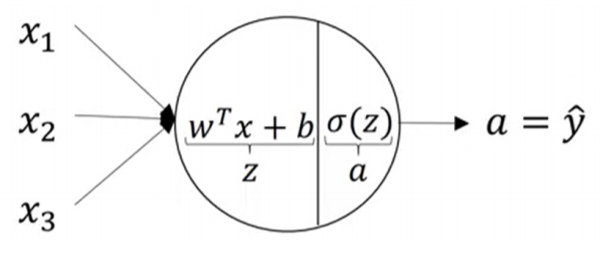
\includegraphics[width=\textwidth]{Figures/Perceptron.png}
    \rule{35em}{0.5pt}
  \caption[Schema of a perceptron]{Schema of a perceptron}
  \label{fig:Perceptron}
\end{figure}


During the backpropagation, the gradient descent algorithm is applied. The aim of the classification process is to minimize the cost. The cost is the average of all the losses which represent the errors between the predictions of the model and the real labels of the pictures. To minimize this cost, we can transform the training task of the ANN into an optimization problem by using a gradient descent, which is a local search algorithm. This algorithm is be used to find the local minimum for a differentiable function. This local minimum corresponds to the state where the model has the best accuracy. Thereby, the process goes backward in the network to update the weights and the bias to decrease the cost and so the number of errors by applying learning rules. 

This algorithm is repeated until the cost has converged.

Let's suppose we want to recognize if a picture contains a cat (label 1) or not (label 0), we can use in the output layer, the activation function sigmoid which returns a value between 0 and 1.

\begin{equation}
{\hat{y}} = {sigmoid(Z)}=\frac{1}{1+e^{-Z} }
\end{equation}
where:

$\hat{y}$ is the label prediction made by the neuron

The predicted label is then set as 1 if the output of the function \emph{sigmoid} is above a treshold, for example 0,5. There are a lot of different activation functions and they are chosen regarding the nature of the task. 




\subsection{Multi-layer perceptron}

Like the previous architecture, multi-layer perceptron is composed by an input and an output layer and also one or several hidden layers. Each hidden layer contains a specific number of nodes. In this architecture, each node is connected to every node in the adjacent layers but not to the nodes in the same layer. This type of connections where the data flow in one direction is called feedforward, there is no recursivity. 

During the forward propagation, the hidden layers apply activation functions on their inputs and transmit the information between the input and the output layer.



\begin{figure}[H]
  \centering
    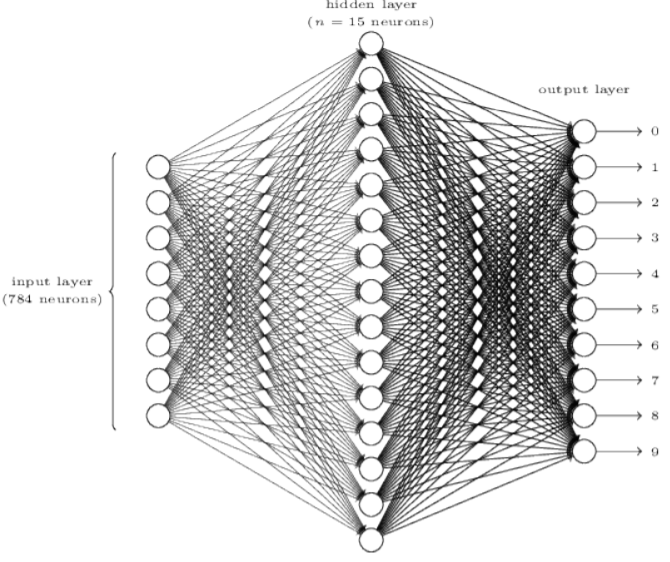
\includegraphics[width=\textwidth]{Figures/multi_layer.png}
    \rule{35em}{0.5pt}
  \caption[Schema of a multi-layer perceptron]{Schema of a multi-layer perceptron with one hidden layer composed by 15 neurons for a classification task involving 10 differents classes}
  \label{fig:Muli-layer perceptron}
\end{figure}

The reason to use this kind of architecture is that it has been demonstrated standard multi-layer feedforward networks with as few as a single hidden layer and arbitrary bounded and nonconstant activation function can approximate any continuous function \cite{multi}.
Indeed, ANN without hidden units can only produce limited mapping model. During the backpropagation, the learning rules are both applied in the hidden layer(s) and in the output layer and this makes the model performing better for more complex classification tasks.

Let's suppose we want to classify pictures into 10 classes. We can use a multi-layer perceptron which output layer is composed by 10 neurons. The activation function sigmoid can be used for the nodes in the hidden layer but not in the output one. We have to use the softmax activation function which is the corresponding function of sigmoid activation for more than two classes. It assigns decimal probabilities to each class. The sum of these decimals must be 1.0. 

\begin{equation}
{softmax(x)_{j}}=\frac{e^{{Z}_{j}}}{\sum_{i=1}^k e^{Z_{i}} }
\end{equation}

where:

${x}$ is the input picture

${j}$ is any particular class we want to get the probability

${k}$ is the number of classes

${Z}$ is the variable that sum all the input values with their associated weights (see equation 2.1) 

To get the prediction of the model for an input, we simply need to recover the corresponding class to the highest probability returned by \emph{softmax}.

 

\section{Convolutional neural networks}
\subsection{Overview}
Machine learning algorithms are good to process a small amount of data but they don't scale well for a large amount. This is the main reason which explain the elaboration of deep neural networks. A lot of different libraries (Theano, TensorFlow, Torch) and interfaces (Keras, Lasagne, Blocks) have been developed in order to make their implementations easier without a deep understanding of the maths theory, high-level programming skills and avoid potential code issues. 

Convolutional neural network is one of the most famous class of deep neural network which is directly inspired by the primary visual cortex of the brain \cite{CNN}.  

It is a type of feedforward neural network composed by neurons that have learnable weights and biases. This network is very similar to the multi-layer perceptron we have seen just before.

CNNs are designed to process different data types but they are mainly used to analyze two dimensional images. In order to classify an image, the input data will be submitted to a serie of different layers : convolution layers, pooling layers, fully connected layers and then an ouput layer where the activation softmax is used. The convolution and the pooling layers are organized into three dimensions: width, height and depth.

\begin{figure}[H]
  \centering
    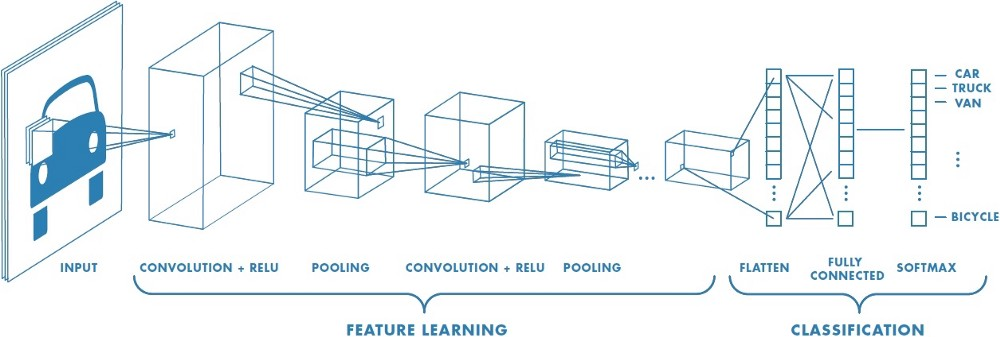
\includegraphics[width=\textwidth]{Figures/convol.jpeg}
    \rule{35em}{0.5pt}
  \caption[Schema of CNN]{Organization of the layers of a convolutional neural networks}
  \label{fig:Muli-layer perceptron}
\end{figure}


CNNs perfom well in image classification because they take into account spatial structure of the image. Indeed, in the convolution layers, each neuron are connected to a small region of the input volume. This region is determined by a matrix called filter. It is then slided over all the inputs to recover a value for the hidden neuron according to a stride. A stride is the size of the step the convolution filter moves each time. For example, a filter of five by five pixels placed in the top left corner of an image layer will be connected to one neuron in the first hidden layer. The filter is then moved to one pixel on the right. This new region will be connected to the second neuron of the first hidden layer. This characteristic is called local collectivity. If the filter does not fit a part of the input image, the picture is padded with zero value pixels or we drop the part of the image where the filter can't be used. 


Filters in convolution layers are used to extract features and so, each hidden neurons in the same layer will share the same weights and bias. In image classification, a feature is an individual measurable property such as edges and objects. This propriety makes CNNs robust to translational invariance. The output of these layers is called feature map. The depth of the features maps generated in the convolutional layer is not fixed and depend of the task we want to perform. For example, if ten filters are used to extract features of an input layer, the depth of the feature map generated will be ten. 

After each convolution layers, an activation function called ReLU is applied. The purpose of this layer is to set all the negative values found in the previous layer to 0. This step makes the network to train much faster.

Then, this rectified feature map will go through a pooling layer in order to reduce its number of dimensions. Pooling extraction is applied on each depth of the feature map. Like in the convolution layer, a filter with as stride is also used in order to separate the feature map into regions.

\begin{figure}[H]
  \centering
    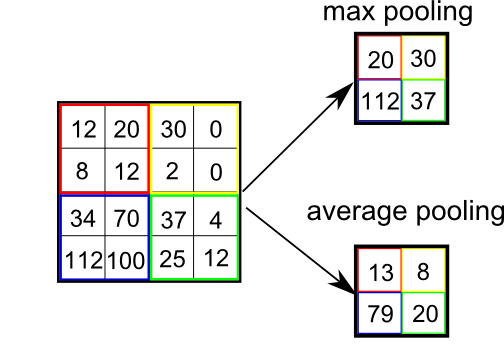
\includegraphics[width=\textwidth]{Figures/pool.png}
    \rule{35em}{0.5pt}
  \caption[Schema of pooling extraction]{Different strategies of pooling extraction using a 2x2 filter and stride 2}
  \label{fig:Muli-layer perceptron}
\end{figure}

Different strategies of pooling extraction exist. The most used ones are max poling where only the highest values of a region is kept and average pooling where the output is the average of all the values in the region. 

The feature maps matrix are then flattened into a vector which feed a fully connected network whose process is the same as described in the previous section of this paper. 


\subsection {AlexNet}
\subsection {VGGNet}
\subsection {GoogLeNet}
\section{Robustness of neural netwoks}


\section{Methods to find adversarial examples}

Different methods have been studied to improve robustness of neural networks \cite{survey}. 
These methods are used to provide guarantee on the safety of networks. Basically an adversarial example can be found by adding to an image natural perturbations such as fog or sunlight. Despite these perturbations, humans will not misclassify the image.

There are three main types of studies concerning adversarial attacks:

- The first one is about non-targeted adversarial attacks. This method consists of modifying the original image to make the network classify it at another random class.

- The second subject area deals with targeted adversarial attacks. This method targets, as its name assumes, one type of class to misclassify it into another precise one.

- The third study concerns defenses against adversarial attacks. This field deals with the problematic of building robust classifiers which are not fooled by adversarial examples. 

Famous methods to find adversarial examples :

- fast gradient sign FGSM

This method is the root of many other methods. The main idea of this method is to add noise to an image at each step of the process to classify an image. Adversarial examples can be easily found on models which use linearity. FSM is based on this assumption and uses the sign or the gradient of the loss function of the model to add or subtract small error to each pixel

- Projected Gradient Descent

This method is a multi-step variant of FGSM and it is why it's more efficient than it. Indeed FGSM is a one-step approach.
It works well for high dimensions cases. 
If a network resist to attacks made with this method, it means it is robust against a lot of other attacks.


- Basic Iterative Method (IBM)

This method is an iterative version of FGSM. This method is more efficient than FGSM because the noise is applied many times instead of once.  Networks which are trained to be robust against one-step adversarial attacks should fail with the attacks made with this method. To avoid put to much noise, the pixel are clipped.


- Carlini-Wagner

This method is able to find each time an adversarial example on defensively distilled and undistilled networks by proposing  3 attacks from 3  different algorithms L0 L2 Linf.  Defensive distillation is a method used to improve the robustness of a network against adversarial examples.

L0 attack  is the first one which manage to find adversarial example one images from the database ImageNet


-Jacobian-based Saliency Map Approach (JSMA)

FSMA is a method  used for targeted misclassification and looks for the smallest perturbation to fool the classification. Compared to the other methods that use output variations to find the related input changes, JSMA builds a map between the input modifications and the output variations. This method is called forward derivative. Like IBM, this method iteratively perturbs features of input data which are the most likely to lead a misclassification with constant offset until the target misclassification is found.

 














%----------------------------------------------------------------------------------------
%	SECTION 2
%----------------------------------------------------------------------------------------

\section{Methods used in Research Papers to evaluate robustness of the neural netwoks}
\subsection {DLV}
\subsection {Two-player game}
\subsection {DeepPoly}

 
%\input{Chapters/Chapter3}
%\input{Chapters/Chapter4} 
%\input{Chapters/Chapter5} 
%\input{Chapters/Chapter6} 
%\input{Chapters/Chapter7} 

%----------------------------------------------------------------------------------------
%	THESIS CONTENT - APPENDICES
%----------------------------------------------------------------------------------------

\addtocontents{toc}{\vspace{2em}} % Add a gap in the Contents, for aesthetics

\appendix % Cue to tell LaTeX that the following 'chapters' are Appendices

% Include the appendices of the thesis as separate files from the Appendices folder
% Uncomment the lines as you write the Appendices

% Appendix A

\chapter{Appendix Title Here} % Main appendix title

\label{AppendixA} % For referencing this appendix elsewhere, use \ref{AppendixA}

\lhead{Appendix A. \emph{Appendix Title Here}} % This is for the header on each page - perhaps a shortened title

Write your Appendix content here.
%\input{Appendices/AppendixB}
%\input{Appendices/AppendixC}

\addtocontents{toc}{\vspace{2em}} % Add a gap in the Contents, for aesthetics

\backmatter

%----------------------------------------------------------------------------------------
%	BIBLIOGRAPHY
%----------------------------------------------------------------------------------------

\label{Bibliography}

\lhead{\emph{Bibliography}} % Change the page header to say "Bibliography"

\bibliographystyle{ieeetr} % Use the "apalike" BibTeX style for formatting the Bibliography

\bibliography{Bibliography} % The references (bibliography) information are stored in the file named "Bibliography.bib"


\end{document}